\chapter{协议实现和性能分析}
\section {协议实现}
\subsection{协议流程}
%    \begin{algorithm}  
%    	\caption{Calculate $y = x^n$}   
%    	\label{alg1}  
%   	\begin{algorithmic} 	 
%    		\REQUIRE $n \geq 0 \vee x \neq 0$   
%    		\ENSURE $y = x^n$   
%    		\STATE $y \Leftarrow 1$   
%    		\IF{$n < 0$}   
%    		\STATE $X \Leftarrow 1 / x$   
%   		\STATE $N \Leftarrow -n$   
%    		\ELSE   
%    		\STATE $X \Leftarrow x$   
%    		\STATE $N \Leftarrow n$  
%    		\ENDIF   
%    		\WHILE{$N \neq 0$}   
%   		\IF{$N$ is even}   
%    		\STATE $X \Leftarrow X \times X$   
%    		\STATE $N \Leftarrow N / 2$   
%    		\ELSE[$N$ is odd]   
%    		\STATE $y \Leftarrow y \times X$   
%    		\STATE $N \Leftarrow N - 1$   
%    		\ENDIF   
%    		\ENDWHILE  
%    	\end{algorithmic}  
%    \end{algorithm}  
MAPA-MACA-CAMA协议的实现是通过节点状态的改变来推进的。节点的接收状态分为三种,分别为IDLE,RECV,COLL状态。节点的发送状态分为五种,分别为RTS、CTS、SEND、ACK状态。通过对比自身的状态和接收到的数据帧的类型,节点可以确定自己在整个传输流程中的位置,进而改变自己的下一步状态。除去等待接收数据帧触发状态改变外,还可以通过定时器超时来改变节点的状态,推进协议的继续。
\paragraph{接收状态}
接收状态的改变是对真实物理环境的一个模拟,在网络仿真中,接收条件的模拟由物理层模拟来实现,这在第六章中会具体解释。
 \begin{figure}[!ht]
 	\centering
 	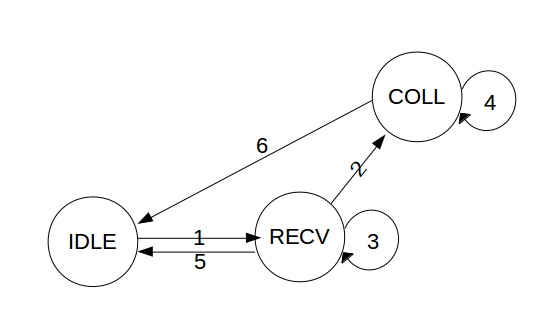
\includegraphics[scale=0.4]{figures/rxstate.png}
 	\caption{
 		rxstate
 	}
 	\label{fig:example}
 \end{figure}
 
\begin{table}[!ht]
	\centering
\begin{tabular}{c p{7cm} p{8cm}}
	\hline  % 在表格最上方绘制横线
	 &状态转移条件&执行的操作\\
	\hline  % 在表格最上方绘制横线
	1&节点空闲状态下侦听到包 & 接收包到pktRx\_\\
	2&节点接收状态下收到其他包,不满足接收条件&节点状态置为冲突状态,清空pktRx\_\\
	3&在接收状态下收到其他包,满足接收条件&节点设置NAV推迟接入,接收新包到pktRx\_,接收完毕后节点状态置为空闲\\
	4&在冲突状态下收到其他包,不满足接收条件&节点状态仍为冲突状态,清空pktRx\_\\
	5&在接收状态下接收完到达包以后&节点状态置为空闲\\	
	6&在冲突状态下收到其他包,满足接收条件&节点设置NAV推迟接入,接收新包到pktRx\_,接收完毕后节点状态置为空闲\\
	\hline
\end{tabular}
\end{table}

\paragraph{发送状态} 发送状态的改变是整个协议的核心流程。图展示了发送状态的转移情况。
 \begin{figure}[!ht]
 	\centering
 	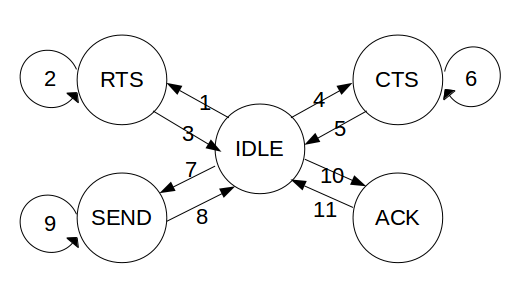
\includegraphics[scale=0.5]{figures/txstate.png}
 	\caption{
 		txstate
 	}
 	\label{fig:example}
 \end{figure}
 
\begin{table}[!ht]
	\centering
	\begin{tabular}{c p{7cm} p{8cm} }
		\hline  % 在表格最上方绘制横线
		&状态转移条件&执行的操作\\
		\hline  % 在表格最上方绘制横线
		1&节点准备开始一次数据传输 &准备pktRTS\_、pktTx\_,节点状态置为RTS\\
		2&RTS状态下接收到RTS、DATA、ACK、BCT包&节点状态不变,丢弃除BCT以外的接收到的包\\
		3&RTS状态下接收到CTS包清空pktRTS\_后或RTS状态超时&发送状态置为空闲,开始下一次发送\\
		4&接收完RTS包,发送状态空闲&准备pktCTRL\_,发送状态置为CTS,发送CTS包\\
		5&CTS状态下接收到DATA包清空pktCTRL\_后或CTS状态超时&发送状态置为空闲,开始下一次发送\\
		6&CTS状态下接收到RTS、CTS、ACK、BCT包&节点状态不变,丢弃除BCT以外的接收到的包\\
		7&接收完CTS包,发送状态空闲&准备pktTx\_发送状态置为MAC\_SEND,发送DATA包\\
		8&SEND状态下接收到ACK包清空pktTx\_后或SEND状态超时&发送状态置为空闲,开始下一次发送\\
		9&SEND状态下接收到RTS、CTS、DATA、BCT包&节点状态不变,丢弃除BCT以外的接收到的包\\
		10&接收完DATA包,发送状态空闲&准备pktCTRL\_,发送状态置为ACK,发送ACK包\\
		11&ACK发送完成&发送状态置为空闲,开始下一次发送\\
		\hline
	\end{tabular}
\end{table}

\subsection{帧格式}
协议共有两种类型的帧数据帧和控制帧。数据帧是网络中所传输数据的载体。控制帧负责广播信息的发送,信道的预约,区域的清空,以及收到数据时的确认等等职责。
\subsubsection{数据帧}
数据帧主要包括帧控制字段、持续期字段、地址字段、序号控制、帧实体和帧校验。其数据帧格式如图所示:
\begin{figure}[!ht]
	\centering
	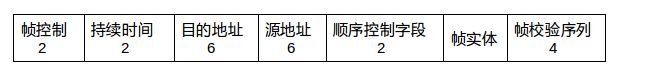
\includegraphics[scale=0.5]{figures/data.png}
	\caption{
		数据帧格式
	}
	\label{fig:example}
\end{figure}
帧控制字段说明MAC协议的版本、使用帧的类型、是否为分布式系统、是
否重传等一些有关数据帧的控制信息。其中的subtype位,1011代表RTS,1100 CTS,1101代表ACK,1110代表BCT。
持续期字段用来记录网络分配矢量NAV(NetworkAllocation Vector)的值。该值主要限定媒介访问时间,提醒其它节点退避。
地址字段有两种地址。目的地址是最后的接收端,源地址是传送的来源。
帧主体字段是帧的数据部分。帧校验序列,用来检查所收到帧的完整性

\subsubsection{控制帧}
BCT帧主要包括帧控制字段、持续期字段、地址字段、负载情况、发送时间和帧校验。BCT帧格式如图所示:
\begin{figure}[!ht]
	\centering
	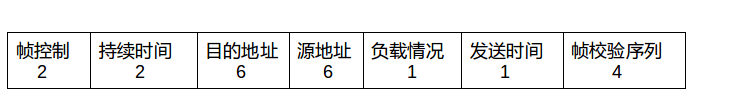
\includegraphics[scale=0.5]{figures/bct.png}
	\caption{
		BCT格式
	}
	\label{fig:example}
\end{figure}
负载情况用于通知固定节点转变数据传输模式,发送时间用于固定节点计算与移动节点之间的距离。

RTS(请求发送)、CTS(清除发送)、ACK(确认帧),主要协助数据帧的传递,管理无线媒介的访问以及提供MAC层的可靠性。格式如下:
\begin{figure}[!ht]
	\centering
	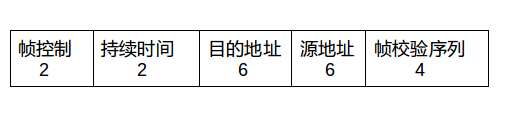
\includegraphics[scale=0.5]{figures/ctrl.png}
	\caption{
		RTS/CTS/ACK格式
	}
	\label{fig:example}
\end{figure}


\section {性能分析}
按照流量模型,信道时间可以划分为信道繁忙时间和信道空闲时间,信道的平均利用率等于发送有效数据的时间和总时间的比值。
\begin{equation}
S=\frac{\overline U}{\overline O+\overline I}
\end{equation}

其中,$\overline U$表示发送有效数据传输时间的期望值,$\overline O$表示信道繁忙时间的期望值,$\overline I$表示信道空闲时间的期望值。
	
\subsection {低负载模式}
在MAPA-CSMA协议中,隐藏终端传输的RTS帧和移动节点定时发送的BCT帧会引起冲突。对于第一种情况,移动节点$\alpha$是固定节点$\omega$和固定节点$\beta$的邻居节点,节点$\beta$是节点$\omega$的隐藏终端。节点$\alpha$在和节点$\omega$进行数据交互的过程中,节点$\beta$发送的RTS帧可能会使得节点$\alpha$接收$\omega$的RTS帧和DATA帧产生碰撞。第二种情况中,除$\alpha$以外的其他邻居移动节点发送的BCT帧会对$\omega$接收CTS和ACK帧产生碰撞。

\begin{figure}[!ht]
	\centering
	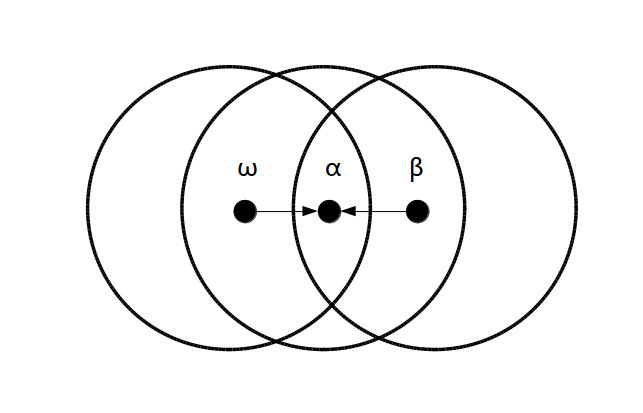
\includegraphics[scale=0.2]{figures/hidden.png}
	\caption{
		数据帧格式
	}
	\label{fig:example}
\end{figure}

假设$P_S$是信道传输的成功概率,也就是在节点$\omega$数据交互周期内没有发生包碰撞的概率。节点$\omega$的邻居节点数量为M。$\omega$邻居移动节点的隐藏终端数量假设为Q,其中固定终端数量为$Q_s$,移动终端为$Q_m$。任一隐藏终端以$\lambda$的速率向移动节点$\alpha$发送RTS包。移动节点$\alpha$以$\mu$的速率定时发送BCT包。

随机退避时间$CW_{min}=W$,$CW_{max}=2_r W$,在第i阶段的退避过程中可随机选择的退避时间为:
\begin{equation}
W_i=2^iW_i \ \ \ i\in(0,r)
\end{equation}
为了简化模型,只考虑第一阶段的退避过程,可选择的退避时间为$(0,W)$。

节点以$\lambda$的速率产生数据,信道传输成功概率是节点在传输数据时邻居节点和隐藏终端不产生干扰的概率:
\begin{equation}
P_S=\lambda(1-\lambda)^{M+Q_s}(1-\mu)^{Q_m}
\end{equation}

节点推迟接入包括接收到邻居节点的RTS帧和接收到邻居节点响应隐藏终端RTS帧而发送的CTS帧,因收到RTS帧推迟接入的概率为:
\begin{equation}
 P_{Rdefer}=(1-\lambda)\lambda M
\end{equation}
因收到CTS帧推迟接入的概率为:
\begin{equation}
 P_{Cdefer}=(1-\lambda)\lambda Q
\end{equation}

一个失败周期的持续时间是等待发送RTS帧的时间和发送RTS未收到CTS回复的超时时间,设最大传输时延为$\tau$,一个失败周期的持续时间为:
\begin{equation}
\begin{aligned}
T_{fail}&=T_{DIFS}+\overline W+Tout_{RTS}\\
&=T_{DIFS}+\overline W+T_{RTS}+2\tau+T_{SIFS}+T_{CTS}
\end{aligned}
\end{equation}

一个成功周期的持续时间包括了RTS,CTS,DATA和ACK的一整个流程,一个成功周期的持续时间为:
\begin{equation}
T_{suc}=T_{DIFS}+\overline W+T_{RTS}+T_{CTS}+T_{DATA}+T_{ACK}+4\tau+3T_{SIFS}
\end{equation}

因收到RTS帧推迟接入的时间为:
\begin{equation}
T_{Rdefer}=T_{CTS}+T_{DATA}+T_{ACK}+3\tau+3T_{SIFS}
\end{equation}

因收到CTS帧推迟接入的时间为:
\begin{equation}
T_{Rdefer}=T_{DATA}+T_{ACK}+2\tau+2T_{SIFS}
\end{equation}

信道繁忙时间为:
\begin{equation}
\overline B=T_{suc}P_S+T_{fail}(\lambda-P_S )+ T_{Cdefer}P_{Cdefer}+T_{Rdefer}P_{Rdefer}
\end{equation}

如果信道繁忙时间大于单位时间,则空闲时间为0;如果信道信道繁忙时间小于单位时间,则除繁忙时间以外的都为空闲时间。空闲时间为:
\begin{equation}
\overline I=\left\{
\begin{aligned}
1-B \ \ \ \ \ \ \ \ B<1\\
0\ \ \ \ \ \ \ \    B\ge 1
\end{aligned}
\right.
\end{equation}

根据吞吐量公式,计算得单一节点的吞吐量$(S)$为
\begin{equation}
\begin{aligned}
S&=\frac{\overline U}{\overline B+\overline I}\\&=\frac{T_{DATA}}{ T_{suc}P_S+T_{fail}(\lambda-P_S )+ T_{Cdefer}P_{Cdefer}+T_{Rdefer}P_{Rdefer}+\overline I}
\end{aligned}
\end{equation}

\subsection {高负载模式}
高负载模式下,节点以$\lambda$的速率产生数据,但是开始一次传输的速率为$\frac{\lambda}{2}$,则信道传输成功概率变为:
\begin{equation}
P_S^h=\frac{\lambda}{2}(1-\frac{\lambda}{2})^{M+Q_s}(1-\mu)^{Q_m}
\end{equation}

因收到RTS帧推迟接入的概率变为:
\begin{equation}
P_{Rdefer}^h=(1-\frac{\lambda}{2})\cdot\frac{\lambda}{2} M
\end{equation}
因收到CTS帧推迟接入的概率变为:
\begin{equation}
P_{Cdefer}^h=(1-\frac{\lambda}{2})\cdot\frac{\lambda}{2} Q
\end{equation}

因为一个失败周期的持续时间是等待发送RTS帧的时间和发送RTS未收到CTS回复的超时时间,高负载模式下超时时间比低负载模式多了一次SIFS等待时间和DATA传输的时间。一个失败周期的持续时间变为:
\begin{equation}
\begin{aligned}
T_{fail}^h&=T_{DIFS}+\overline W+Tout_{RTS}\\
&=T_{DIFS}+\overline W+T_{RTS}+2\tau+T_{SIFS}+T_{CTS}
\end{aligned}
\end{equation}

一个成功周期的持续时间则包括了RTS,CTS,2DATA和ACK的一整个流程,一个成功周期的持续时间变为:
\begin{equation}
T_{suc}^h=T_{DIFS}+\overline W+T_{RTS}+T_{CTS}+2T_{DATA}+T_{ACK}+4\tau+4T_{SIFS}
\end{equation}

因收到RTS帧推迟接入的时间变为
\begin{equation}
T_{Rdefer}^h=T_{CTS}+2T_{DATA}+T_{ACK}+3\tau+4T_{SIFS}
\end{equation}

因收到CTS帧推迟接入的时间变为
\begin{equation}
T_{Rdefer}^h=2T_{DATA}+T_{ACK}+2\tau+2T_{SIFS}
\end{equation}

信道繁忙时间为:
\begin{equation}
\overline B^h=T_{Cdefer}^hP_{Cdefer}^h+T_{Rdefer}^hP_{Rdefer}^h
\end{equation}

信道空闲时间为:
\begin{equation}
\overline I^h=\left\{
\begin{aligned}
1-\overline B^h \ \ \ \ \ \ \ \ B<1\\
0\ \ \ \ \ \ \ \    B\ge 1
\end{aligned}
\right.
\end{equation}

根据吞吐量公式,计算得单一节点的吞吐量$(S)$为
\begin{equation}
\begin{aligned}
S^h&=\frac{\overline U^h}{\overline B^h+\overline I^h}\\&=\frac{2T_{DATA}}{ T_{suc}^h P_S^h+T_{fail}^h(\frac{\lambda}{2}-P_S^h )+ T_{Cdefer}^hP_{Cdefer}^h+T_{Rdefer}^hP_{Rdefer}^h+\overline I^h}
\end{aligned}
\end{equation}

\endinput